\label{sec:threat}

\subsection{Smart Grid Attack Surface}

Figure~\ref{fig:sysoverview} depicts the target environment. Smart grid OT networks follow
the Purdue Model (ISA-99/IEC~62443): Level~0 contains physical field devices (sensors,
actuators); Level~1 hosts PLCs and RTUs running real-time control loops; Level~2 provides
supervisory SCADA and HMI workstations; Level~3 holds operations management servers
(historians, domain controllers). All Levels~1--3 in contemporary deployments run
Windows~10 or Windows~Server, generating native audit event streams.

\begin{figure}[!t]
  \centering
  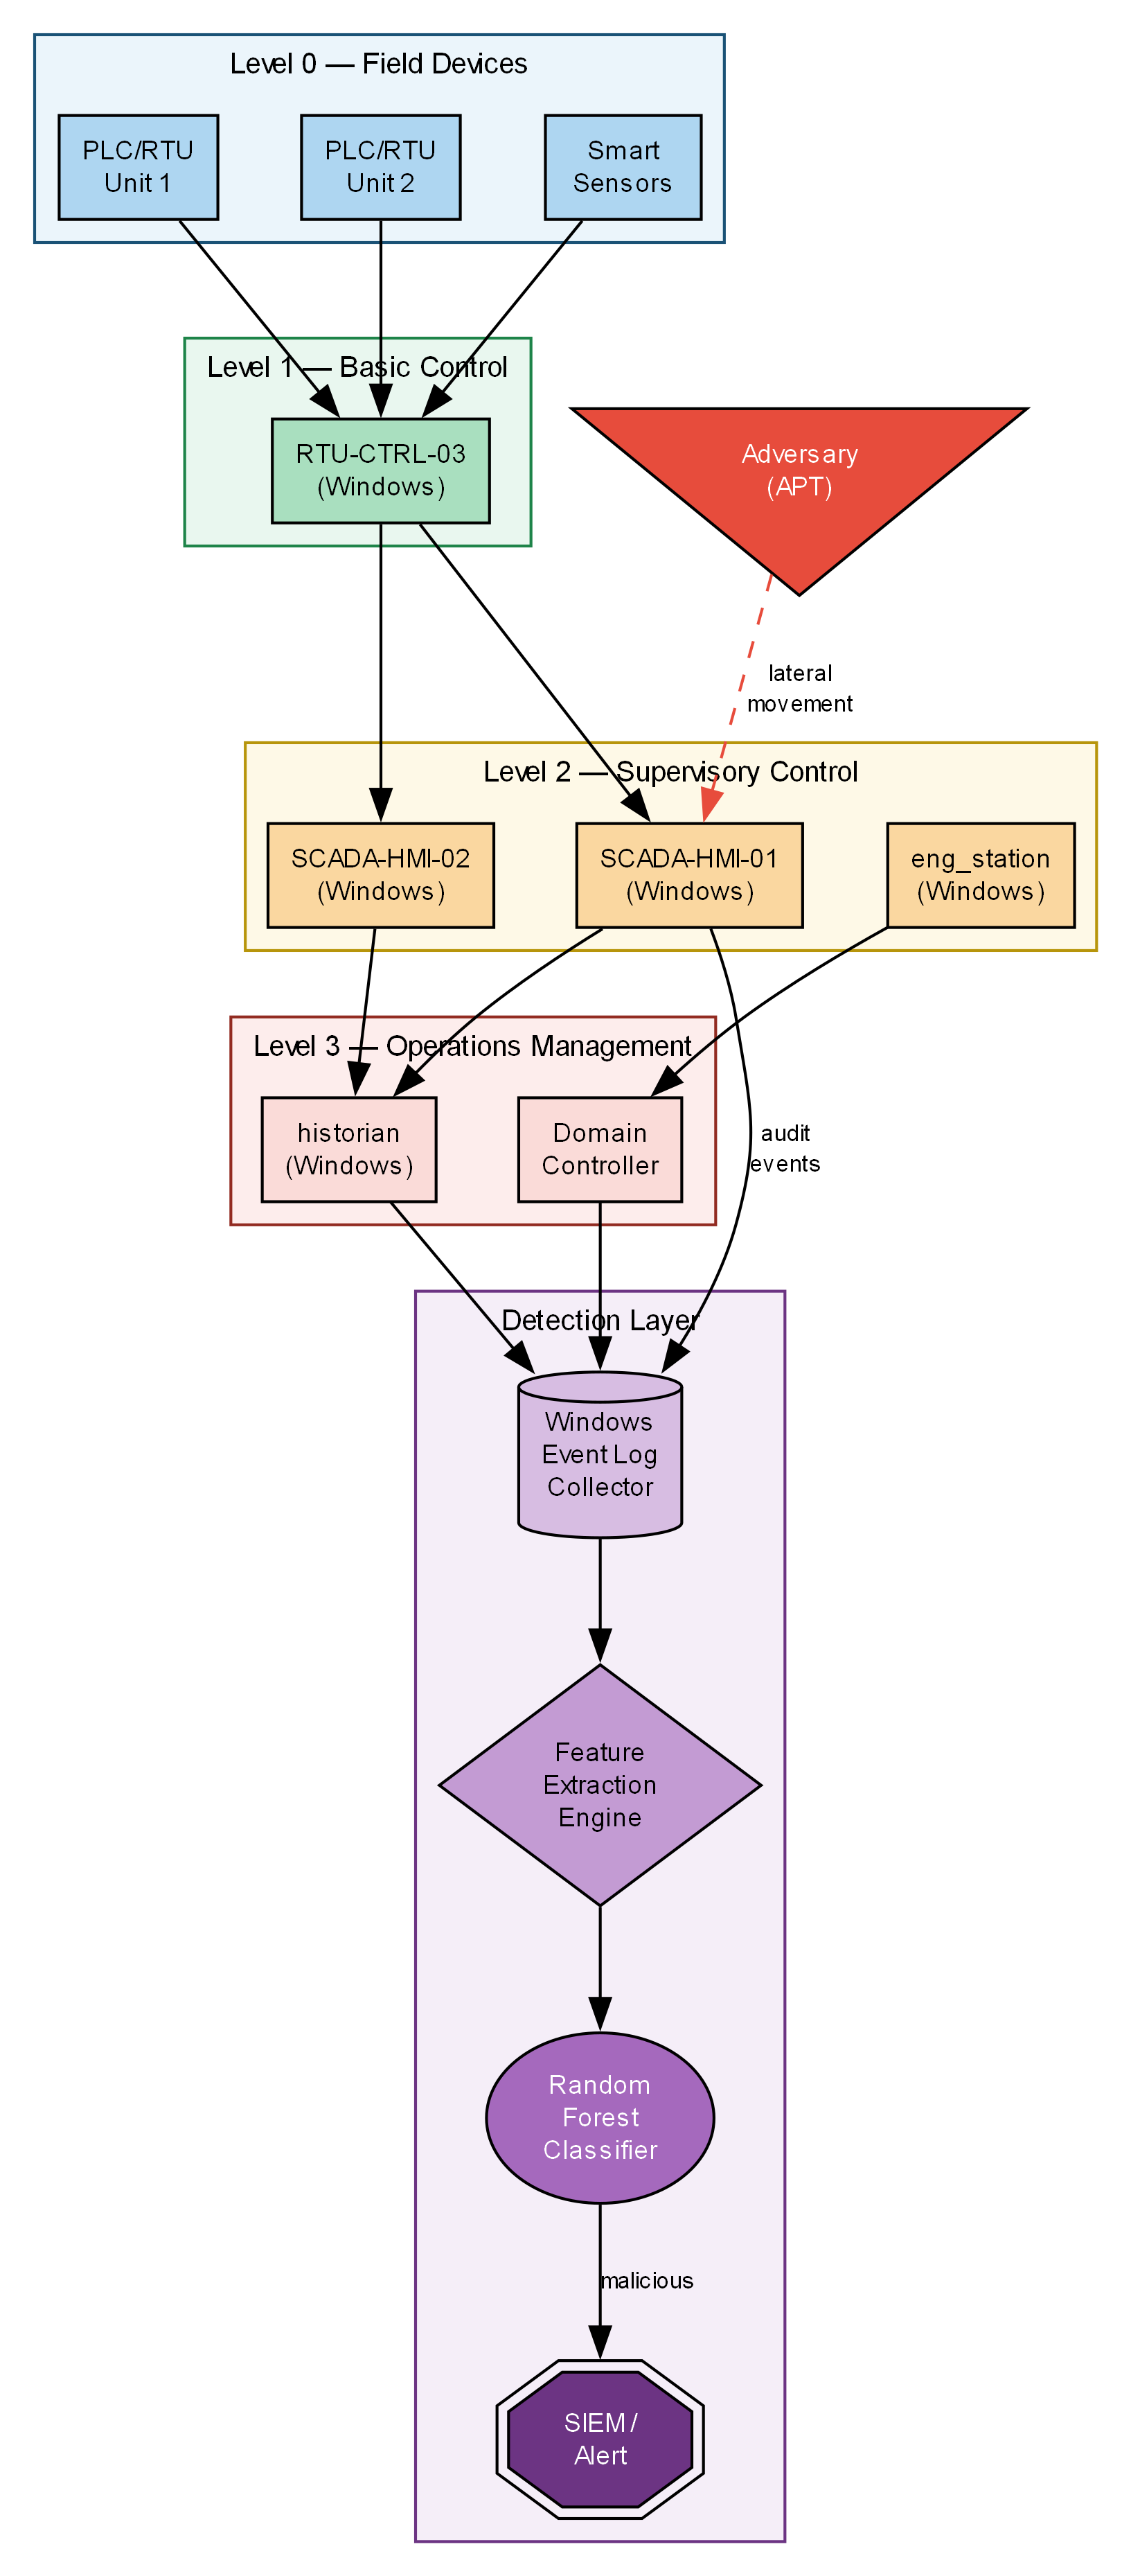
\includegraphics[width=\columnwidth]{figs/system_overview.png}
  \caption{Target environment: smart grid Purdue model levels and detection layer placement.}
  \label{fig:sysoverview}
\end{figure}

\subsection{Attacker Model}

We adopt a conservative but realistic adversary model aligned with MITRE ATT\&CK for
ICS \cite{mitre2020attack}:

\textbf{Goals.} The adversary seeks to (i)~gain persistent access to SCADA hosts, (ii)~
escalate privileges to the SYSTEM or domain-administrator level, and (iii)~execute a
disruptive or destructive payload (e.g., rogue command injection, service disruption).
Detection and evasion of security monitoring are secondary goals.

\textbf{Capabilities.} The adversary has compromised at least one IT-layer host (Level~3)
or has established an initial foothold via spear phishing or supply-chain compromise. They
possess valid or cracked domain credentials. Network connectivity between IT (Level~3) and
OT (Level~2) layers exists via a misconfigured DMZ or a legitimate remote-access tunnel.

\textbf{Access assumptions.} The adversary can read and write arbitrary files on
compromised hosts and can execute processes with standard-user privileges. Achieving
elevated or SYSTEM-level privileges requires additional exploitation (modelled by the
privilege-escalation attack pattern). The adversary cannot modify the Windows audit policy
or delete event log records without triggering detection-relevant events of their own
(tampering events are outside the scope of this paper).

\subsection{Attack Patterns Modelled}

Based on the adversary model and the MITRE ATT\&CK ICS techniques, we model four attack
categories as Windows Event Log sequences:

\begin{enumerate}
  \item \textbf{Lateral movement} (T0812, T0866): password-spraying attempts (repeated
        event~4625) followed by a successful logon (4624) from an unexpected source IP,
        targeting SCADA HMI or RTU hosts.

  \item \textbf{Persistence} (T0873): installation of a malicious service (event~7045)
        followed immediately by service start (7036) and process creation (4688) with an
        unusual binary name.

  \item \textbf{Privilege escalation} (T0890): a special-privileges logon (event~4672)
        immediately preceding process creation (4688) of a known offensive tool
        (\texttt{mimikatz.exe}, \texttt{psexec.exe}).

  \item \textbf{Reconnaissance} (T0840, T0843): a rapid burst of object-access attempts
        (event~4663) on HMI or RTU file systems, targeting configuration files and setpoint
        databases within a compressed time window ($<30$~seconds).
\end{enumerate}

\subsection{Detection Scope and Assumptions}

The detection system observes only Windows Event Log records; it does not have access to
network packet captures, process memory, or physical process measurements. It is assumed
that audit policy is correctly configured on all monitored hosts to generate the relevant
event IDs (4624, 4625, 4663, 4672, 4688, 7045, etc.), consistent with NERC CIP-007-6
requirements. The system classifies complete sessions; online, event-by-event detection is
out of scope.
